\documentclass[12pt]{article}
\usepackage{graphicx}
\usepackage{amsmath}
\usepackage{mathtools}
\usepackage{gensymb}

\newcommand{\mydet}[1]{\ensuremath{\begin{vmatrix}#1\end{vmatrix}}}
\providecommand{\brak}[1]{\ensuremath{\left(#1\right)}}
\providecommand{\norm}[1]{\left\lVert#1\right\rVert}
\providecommand{\abs}[1]{\left\vert#1\right\vert}
\newcommand{\solution}{\noindent \textbf{Solution: }}
\newcommand{\myvec}[1]{\ensuremath{\begin{pmatrix}#1\end{pmatrix}}}
\let\vec\mathbf

\begin{document}
\begin{center}
\textbf\large{CONIC SECTIONS}

\end{center}
\section*{Excercise 11.4}
Q2.Find the coordinates of the focii, the vertices, the eccentricity and the length of the latus rectum of a hyperbola whose equation is given by $\frac{y^2}{9}-\frac{x^2}{27}=1$.
\solution
The equation of the hyperbola can be rearranged as
\begin{align}
	\label{eq:eq1}
	-x^2 + 3y^2 -27 = 0
\end{align}
The above equation can be equaded to the generic equation of conic sections
\begin{align}
	\label{eq:eq2}
	g\brak{\vec{x}}=\vec{x}^\top \vec{V} \vec{x} + 2\vec{u}^\top \vec{x} + f = 0
\end{align}
Comparing coefficients of both equations \eqref{eq:eq1} and \eqref{eq:eq2}
\begin{align}
	\label{eq:eq3}
	\vec{V} &= \myvec{-1&0\\0&3}\\
	\vec{u} &= \vec{0}\\
	f &= -27
\end{align}
From equation \eqref{eq:eq3}, since $\vec{V}$ is already diagonalized, the eigen values $\lambda_1 \text{ and } \lambda_2$ are given as
\begin{align}
	\lambda_1 &= -1\\
	\lambda_2 &= 3
\end{align}
\begin{enumerate}
\item The eccentricity of the hyperbola is given as
\begin{align}
	e &= \sqrt{1 - \frac{\lambda_2}{\lambda_1}} = \sqrt{1+\frac{3}{1}}\\
	  &= 2
\end{align}
\item For the standard hyperbola, the coordinates of Focii are given as
\begin{align}
	\label{eq:eq4}
	\vec{F} = \pm \frac{\brak{\frac{1}{e\sqrt{1-e^2}}}\brak{e^2}\sqrt{\frac{\lambda_1}{f_0}}}{\frac{\lambda_1}{f_0}} \vec{e}_2
\end{align}
where
\begin{align}
	f_0 &= -f\\
	\eqref{eq:eq4} \implies &= \pm \frac{\brak{\frac{1}{2\sqrt{1-4}}}\brak{4}\sqrt{\frac{-1}{27}}}{\frac{-1}{27}} \vec{e}_2\\
	&= \pm \myvec{0\\6}
\end{align}
\item The vertices of the hyperbola are given by
\begin{align}
	\pm \myvec{0\\\sqrt{\abs{\frac{f_0}{\lambda_2}}}}= \pm \myvec{0\\3}
\end{align}
\item The length of latus rectum is given as
\begin{align}
	2\frac{\sqrt{\abs{f_0 \lambda_2}}}{\lambda_1} &= 2\frac{\sqrt{\abs{27\brak{3}}}}{-1}\\
	&= 18
\end{align}
as length cannot be negative
\end{enumerate}
The corresponding is shown in Figure \ref{fig:Fig1}
\begin{figure}[!h]
	\begin{center} 
	    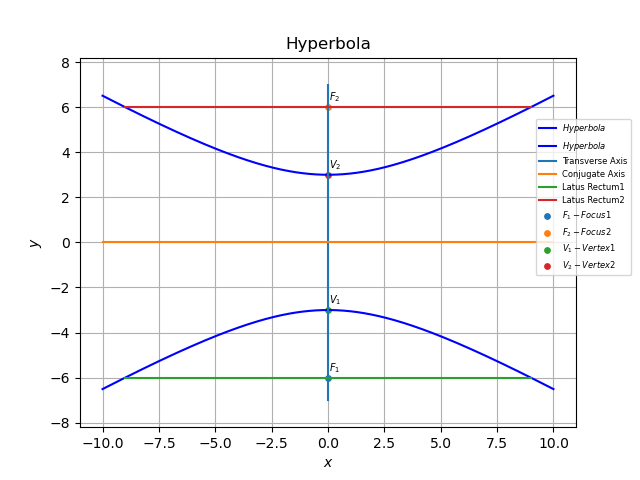
\includegraphics[width=\columnwidth]{figs/hyperbola}
	\end{center}
\caption{}
\label{fig:Fig1}
\end{figure}

\end{document}


